Die Prüfung des Dokuments erfolgt im ersten Schritt auf Echtheit des öffentlichen Schlüssels mittels der Identifizierungsnummer und des Namens der Zertifizierungsstelle aus dem übermittelten Zertifikat. Im nächsten Schritt wird die Prüfung des Zertifikates mithilfe des öffentlichen Schlüssels aus der öffentlich, zugänglichen Datenbank der Zertifizierungsstelle durchgeführt. Ist die Echtheit sichergestellt wird die Entschüsselung der Signatur durch den öffentlichen Schlüssel durchgeführt. Das Ergebnis der Entschlüsselung ist der vom Absender erzeugte Fingerabdruck. Als letzter Schritt wird anhand des im Zertifkat genannten Hash-Algorithmus erneut ein Fingerabruck des Dokuments erstellt und mit dem entschlüsselten Fingerabdruck verglichen. Die Unversehrheit des Dokuments ist gewährleistet, wenn die beiden Fingerabdrücke des Dokuments übereinstimmen. \cite{techno1}
\begin{figure}[!ht]
    \centering
    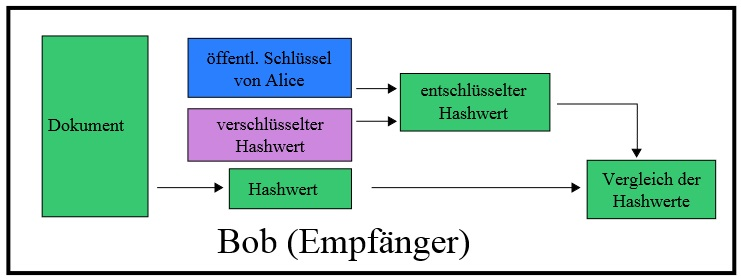
\includegraphics[width=\textwidth]{PruefungEmpfaenger2.jpg}
    \caption[Prüfung eines Dokuments mit digitaler Signatur]{Prüfung eines Dokuments mit digitaler Signatur. \cite{techno3}}
    \label{fig:3}
\end{figure}